%\documentclass[twocolumn]{article}
\documentclass{article}

\usepackage[utf8]{inputenc}

\usepackage{graphicx} 
\usepackage{subfigure}
\usepackage{paralist}
\usepackage{amsfonts}
\usepackage{hyperref}

\usepackage{url}
\usepackage{booktabs}

\usepackage[usenames,dvipsnames]{xcolor}
\usepackage{tikz}
\usetikzlibrary{positioning, calc}

\usepackage[draft,nomargin,footnote]{fixme}

\graphicspath{{figs/}}

\usepackage{xspace}
\newcommand{\eg}{\textit{e.g.}\xspace}
\newcommand{\etal}{\textit{et al.}\xspace}
\newcommand{\ie}{\textit{i.e.}\xspace}
\newcommand{\etc}{\textit{etc.}\xspace}
\newcommand{\vs}{\textit{vs.}\xspace}

\title{Learning by Teaching a Robot:\\The Case of Handwriting}

\author{Séverin Lemaignan$^1$, Alexis Jacq$^{1,2}$, Fernando Garcia$^1$,
    Deanna Hood$^1$, \\Aude
    Billard$^1$, Ana Paiva$^2$, Pierre Dillenbourg$^1$ \\
$^1$CHILI Lab, École Polytechnique Fédérale de Lausanne, Suisse,\\
$^2$Instituto Superior Técnico, University of Lisbon, Portugal}

\begin{document}
\maketitle

%\begin{abstract}
%
%    Robots for education are not limited to support ICT teaching, and they are
%    indeed finding new roles in the classroom. This article reports on such a
%    new paradigm for educative robots, that involves \emph{learning by teaching}
%    and strong \emph{social engagement} to help children struggling with
%    handwriting. Our system relies on machine-learning and child-robot
%    interaction with a small humanoid robot, and we present several real-world
%    studies in schools and with occupational therapists that led us to promising
%    initial results.
%
%\end{abstract}


%%%%%%%%%%%%%%%%%%%%%%%%%%%%%%%%%%%%%%%%%%%%%%%%%%%%%%%%%%%%%%%%%%%%%%%%%%%%%%%%%%%
%%%%%%%%%%%%%%%%%%%%%%%%%%%%%%%%%%%%%%%%%%%%%%%%%%%%%%%%%%%%%%%%%%%%%%%%%%%%%%%%%%%
%%%%%%%%%%%%%%%%%%%%%%%%%%%%%%%%%%%%%%%%%%%%%%%%%%%%%%%%%%%%%%%%%%%%%%%%%%%%%%%%%%%
\section{A Different Paradigm for Educative Robots}

Thomas is five and half, and has been diagnosed with visuo-constructive
deficits. He is under the care of an occupational therapist, and tries to
workaround his inability to draw letters in a consistent manner. Vincent is six
and struggles at school with his poor handwriting and even poorer
self-confidence.\footnote{Children's names have been changed.}

While Thomas is lively and always quick at shifting his attention from one
activity to another, Vincent is shy and poised. Two very different children,
facing however the same difficulty to write in a legible manner. And, hidden
beyond this impaired skill, psycho-social difficulties arise: they
underperform at school, Thomas has to go for follow-up visits every week,
they both live under the label ``requires special care''. This is a source of
anxiety for the children and for their parents alike.

\begin{figure}
    \centering
    \includegraphics[width=0.9\linewidth]{henry}
    \caption{\small Thomas teaching Nao how to write numbers, with the help of an
    occupational therapist.}
    \label{fig:henry}
\end{figure}

Remediations for handwriting difficulties traditionally involve long
interventions (at least 10 weeks~\cite{Hoy2011}), essentially consisting in
handwriting training with occupational therapists, and primarily addressing the
\emph{motor} deficits.  Improvements in self-confidence and anxiety occur (at
best) as a side-effect of the child improving his/her handwriting skills and,
consequently, improving his/her performance at school.

We present in this article a new take on this educative challenge: a remediation
procedure that involve a ``bad writer'' robot that is \emph{taught} by the
child. By building on the \emph{learning by teaching} paradigm, not only the
child practises handwriting but, as (s)he takes on the role of the teacher,
(s)he also positively reinforce his/her self-esteem and motivation: his/her
social role shifts from the ``underperformer'' to ``the one who knows and
teaches''. And by relying on a robot, we can tailor the exercises and the
learning rate to each children' needs, as we show in this article.

\subsection{Learning by Teaching}

The \emph{learning by teaching} paradigm, which engages the student in the act
of teaching another, has been shown to produce motivational, meta-cognitive, and
educational benefits in a range of disciplines~\cite{Rohrbeck2003}. The
application of this paradigm to handwriting intervention remains, however,
unexplored. One reason for this may be due to the requirement of an
appropriately unskilled peer for the child to tutor: this may indeed prove
difficult if the child is the lowest performer in the class.  In some cases, it
may be appropriate for a peer or teacher to simulate a na\"ive learner for the
child to teach. For handwriting however, where one's skill level is visually
evident, this acting is likely to be rapidly detected. This motivates the use of
an artificial teachable agent which can be configured for a variety of skill
levels, and for which children do not have preconceptions about its handwriting
ability.

Robots have been used as teachers or social partners to promote children's
learning in a range of contexts, most commonly related to language
skills~\cite{han2010robot}, and less often to physical skills (such as
calligraphy~\cite{Matsui2013}). Looking at the converse (humans \emph{teaching}
robots), Werfel notes in~\cite{Werfel2014} that most of the work focuses on the
robot's benefits (in terms of language~\cite{Saunders2010} or
physical~\cite{Mulling2013} skills, for example) rather than the learning
experienced by the human tutor themselves.  Our work concentrates on this latter
aspect: by demonstrating handwriting to a robot, we aim at improving the
\emph{child's} performance. Note that our work must be distinguished from
``learning from demonstration'' approaches to robots learning physical skills,
as the agent we present is only simulating fine motor skills for interaction
purposes.

A robotic learning agent which employs the learning by teaching paradigm has
previously been developed by Tanaka and Matsuzoe~\cite{Tanaka2012}. In their
system, children learn vocabulary by teaching the {\sc nao} robot to act out
verbs. The robot is tele-operated (Wizard-Of-Oz) and mimics the actions that the
children teach it, but with no long-term memory or learning algorithm in place.
Our project significantly extends this line of work in two ways. First, by
investigating the context of children's acquisition of a challenging physical
skill (handwriting), and second by proposing a robotic partner which is fully
autonomous in its learning.

\subsection{Agency and Commitment}

We also investigate here a particular role for a robot in the
education of handwriting: not only is the robot actively performing the activity
by drawing letters, but it does so in a way that engages the child in a very
specific social role. The child is the teacher in this relationship and the
robot is the learner: the child must engage in a (meta-) cognitive relationship
with the robot to try to understand why the robot fails and how to help it best.
Here, the robot is more than just an activity facilitator or orchestrator -- its
physical presence and embodiment induce agency and anthropomorphising, and
cognitively engage the child into the learning activity (be it consciously or
not).

Besides the commitment of the child into the interaction build on a
psychological effect known as the
``protégé effect''~\cite{Chase2009}: the teacher feels responsible for his student, commits
to the student's success and possibly experiences student's failure as his own
failure to teach. Teachable computer-based agents have previously been used to
encourage this ``protégé effect'', wherein students invest more effort into
learning when it is for a teachable agent than for themselves~\cite{Chase2009}.
We rely on this cognitive mechanism to reinforce the child's commitment into the
robot-mediated handwriting activity, and we indeed show sustained child-robot
engagement over extended periods of time (several hours spread of a month).

For these two reasons, our approach is to be distinguished from previous works in
educational robotic. Most of these do not consider the agency induced by the
robot beyond its motivational aspect: playing with an interactive, partially autonomous
device naturally induces some form of anthropomorphizing, which leads to some
level of projected agency, and participate the overall excitement (at least, on
the short-term, before the novelty effect vanishes).

In our case, the role of agency is stronger: it induces meta-cognition (``I am
interacting with an agent, so I need to reflect on how to best teach him'')
which is beneficial for the learning process; it also induces a protégé
effect (``I want my robot-agent to succeed!'') which support the commitment of
child into the interaction, also for longer period of time.


Building on these socio-cognitive mechanisms, our intent is therefore to design
a robotic system that would effectively support handwriting remediation in an
original way: by getting children to teach a robotic agent how to write, those
children would both practise without knowing it and recover self-confidence and
self-esteem by supporting a worst-than-themselves robotic ``student''.

The following sections of the paper go into details. We first provides a
brief overview of the robotic system and the interaction it induces. We also
present the machine-learning techniques that allow the robot to learn
from the children, followed by the implementation on a {\sc nao} robot.

We then present and report on the field experiments that we conducted over the
last two years, including four studies at school, one longer experiment
with eight children at the surgery of an occupational therapist, and two
one-month long case studies. While the focus of the school
experiments was mostly technical validation and data acquisition, the three
other experiments involved children with actual deficits, and gave us initial insights on the
relevance and effectiveness of our approach.

%%%%%%%%%%%%%%%%%%%%%%%%%%%%%%%%%%%%%%%%%%%%%%%%%%%%%%%%%%%%%%%%%%%%%%%%%%%%%%%%%%%
%%%%%%%%%%%%%%%%%%%%%%%%%%%%%%%%%%%%%%%%%%%%%%%%%%%%%%%%%%%%%%%%%%%%%%%%%%%%%%%%%%%
%%%%%%%%%%%%%%%%%%%%%%%%%%%%%%%%%%%%%%%%%%%%%%%%%%%%%%%%%%%%%%%%%%%%%%%%%%%%%%%%%%%
\section{Implementation of the Interaction}

Figure~\ref{experimental_setup} illustrates our general experimental setup: a
face-to-face child-robot interaction with an autonomous Aldebran's {\sc nao}
robot.

A tactile tablet (with a custom application) is used for both the robot and the
child to write: during a typical round, the child requests the robot to write
something (a single letter, a number or a full word), and push the tablet
towards the robot. The robot writes on the tablet by gesturing the writing -- the
letters being actually drawn by the tablet application itself. The child then pull back the
tablet, corrects the robot's attempt by writing him/herself on top or next to
the robot's writing (see Figure~\ref{fig:diego}), and ``send'' his/her
demonstration to the robot by pressing a small button on the tablet. The robot
``learns'' from this demonstration and tries again.

Since the children are assumed to take on the role of the teachers, we had to ensure
they would be able to manage by themselves the turn-taking and the overall
progression of the activity (moving forwards to the next letter or word). In our design,
the turn-taking relies on the robot prompting for feedback once it is done with
its writing (through simple sentences like ``What do you think?''), and pressing on a
small robot icon on the tablet once the child has finished correcting. In our
experiments, both were easy to grasp for children.


\begin{figure}
    \centering
    
\includegraphics[width=0.6\columnwidth]{experimental_setup}
    \caption{\small Our experimental setup: face-to-face interaction with a {\sc
        nao} robot.  The robot writes on the tactile tablet, the child then
        corrects the robot by directly overwriting its letters on the tablet
        with a stylus. An adult (either a therapist or an experimenter,
        depending on the studies), remains next to the child to guide the work
        (prompting, turn taking, etc.). For some studies, a second tablet and an
        additional camera (dashed) are employed.}

    \label{experimental_setup}
\end{figure}

Implementing such a system raises several challenges: first, the acquisition,
analyse and learning from hand-written demonstration, which lays at the core of the
our approach, necessitates the development of several algorithms for the robot to generate
initial bad writing and to respond in an adequate manner, showing visible (but
not too quick) writing improvements.

Then, the actual implementation on the robot requires the coordination of
several modules (from performing gestures and acquiring the user's input to
the state machine implementing the high-level behaviour), spread over several devices (the robot itself,
one laptop and up to four tactile tablets for some of the studies that we conducted). We
relied on ROS to ensure the synchronization and communication between these
modules.

We detail each of these in the following sections.

%%%%%%%%%%%%%%%%%%%%%%%%%%%%%%%%%%%%%%%%%%%%%%%%%%%%%%%%%%%%%%%%%%%%%%%%%%%%%%%%%%%
\subsection{Generating and Learning Letters}

Since our application is about teaching a robot to write, generating (initially
bad) letters and learning from demonstrations is a core aspect of the project.

The main insight for both the generation and the learning of letters is to
reason about the shape of letters in their eigenspace, instead of the natural
cartesian space. The eigenspace of each letters is spanned by the first $n$
eigenvectors (in our experiments, $3 < n < 6$) of the covariance matrix
generated from a standard dataset of adult letters (the UJI Pen Characters 2
dataset~\cite{Llorens2008}).  This procedure, based on a Principle Component
Analysis (PCA), is explained in details in a previously published
article~\cite{hood2015when}.

By changing the eigenvalues associated to these eigenvectors and regenerating
letters with the reverse procedure, it becomes then easy to generate new
letters, with distortions that are actually plausible handwriting errors: they
are actually exaggerations of variance of writing styles that naturally
occurs amongst adult writers.  Figure~\ref{fig:sampleLetters} shows examples of
deformed ``g'' generated with such a technique.

\begin{figure}
    \centering
    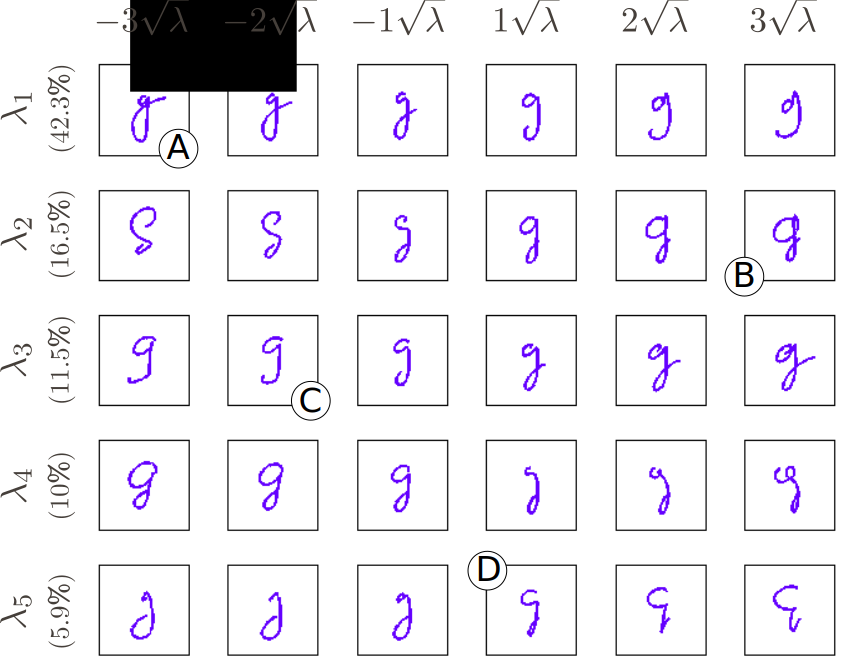
\includegraphics[width=0.9\linewidth]{cowriter-g}
    \caption{\small \label{fig:sampleLetters} \textbf{Generating bad letters}:
        effect of varying the first five eigenvalues (rows) of the shape model
        of ``g'' by different factors (columns). The percentage of the total
        variance in the dataset explained by each eigenvalue is shown      on
        the appropriate row. Examples noted A, B, C, D illustrate how the
        PCA-based approach allows to \emph{automatically} generate letters whose
        errors can be \emph{semantically} interpreted, \eg A has a too large bottom
        loop, B has a wide top loop, the bottom loop of C is not correctly
        closed, the top loop of D is not closed, etc.}

\end{figure}

The same technique can also be applied to \emph{classify} demonstrations,
\emph{assess} their quality and \emph{learn} from them. Figure~\ref{fig:h} shows
for example nine allographs of ``h'' written by a 6 years old child, along with the
mean letter from the dataset (reference letter). By projecting each of the
demonstrations onto the eigenspace of ``h'' (Figure~\ref{fig:h}b), we observe
that:

\begin{itemize}
    \item the different allographs can by clustered (with a $k$-means or
        mean-shift algorithm) by their visual styles,
    \item we can compute an euclidian distance to the reference letter to assess
        the visual proximity of the demonstration with the expected letter, thus
        providing a quantitative metric of writing performance.
\end{itemize}

\begin{figure}[ht!]
    \centering
    \subfigure[Nine allographs of the cursive ``h'', next to the reference]{
        \includegraphics[width=0.45\columnwidth]{h}
    }
    \subfigure[Same samples, normalized and projected in the eigenspace spanned from the
        3 first eigenvectors: clusters arise, that actually match writing styles.]{
        \includegraphics[width=0.45\columnwidth]{eigenspace-uniformization}
    }

    \caption{\small Projecting demonstrated letters onto the eigenspace
    generated from the reference dataset effectively clusters the samples
    according to their topological similarity. Allographs that are similar to
    the reference are close to it in the eigenspace.}
    \label{fig:h}
\end{figure}

The algorithm for machine-learning becomes then a simple matter of converging at
a specific pace towards the child demonstration in the eigenspace.
Figure~\ref{learning_6_demos} (p.~\pageref{learning_6_demos}) illustrates the
process with the complete learning cycle of the number ``6''.

%%%%%%%%%%%%%%%%%%%%%%%%%%%%%%%%%%%%%%%%%%%%%%%%%%%%%%%%%%%%%%%%%%%%%%%%%%%%%%%%%%%
\subsection{Robotic Implementation}

Our system is embodied in an Aldebaran's {\sc nao} (V4 or V5, depending on the
studies) humanoid robot. This choice is motivated by its approachable
design~\cite{Gouaillier2008}, its size (58cm) and inherently safe structure
(lightweight plastic) making it suitable for close interaction with children,
its low price (making it closer to what school may afford in the coming years)
and finally its ease of deployment on the field.

Robotic handwriting requires precise closed-loop control of the arm and hand
motion. Because of the limited fine motor skills possible with such an
affordable robot, in addition to the absence of force feedback, we have opted
for \emph{simulated handwriting}: the robot draws letters in the air, and the
actual writing is displayed on a synchronised tablet.

\begin{figure}[ht!]
\centering

\resizebox{0.7\linewidth}{!}{%

\begin{tikzpicture}[
    >=latex,
    node distance=2cm,
    every edge/.style={draw, very thick},
    redarrow/.style={draw,red, text=black},
    greenarrow/.style={draw,GreenYellow,text=black},
    yellowarrow/.style={draw,BurntOrange,text=black},
    cmpt/.style={draw, align=center, rounded corners, inner sep=5pt, font=\sf, fill=black!20},
    label/.style={midway, align=left, font=\scriptsize\sf, fill=white, above,opacity=0,text opacity=1}]

    \node at (0,0) (laptop) {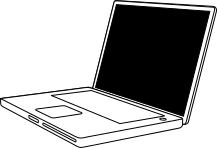
\includegraphics[width=2cm]{laptop}};
    \node[below right=2 of laptop] (nao) {
\includegraphics[width=2cm]{nao}};
    \node[below left=2 of laptop] (tablet) {
\includegraphics[width=2cm]{tablet+stylus}};
    \node[above=2 of laptop] (selection) {
\includegraphics[width=2cm]{selection_tablet}};

    \node[draw,above right=2 of laptop,anchor=north west,text width=4cm] (processes)
    {\sf\scriptsize machine-learning, \\letters/gestures
    generation, \\interaction supervision};
    \path (laptop) edge[dashed] (processes);

    \path (nao) edge [->,redarrow, bend left] node[label, auto] {robot state} (laptop);
    \path (laptop) edge [->,greenarrow, bend left] node[label, auto] {writing gestures} (nao);

    \path (tablet) edge [->,redarrow, bend left] node[label, auto] {demonstrations,\\turn taking} (laptop);
    \path (laptop) edge [->,redarrow, bend left] node[label,
    auto=right,align=right]
    {path of\\ letters to display} (tablet);

    \path (selection) edge [->,redarrow] node[label, auto=right] {letter/word to write} (laptop);

    \path (-5, 2) edge [->, redarrow] node[label] {ROS} ++(1, 0);
    \path (-5, 2.6) edge [->, greenarrow] node[label] {NaoQI} ++(1, 0);
    
\end{tikzpicture}
}

\caption{\small \textbf{Overview of the system}. In total, the system runs about 10 ROS nodes,
    distributed over the robot itself, a central laptop and Android tablets.}

    \label{fig:archi}
\end{figure}

The overall architecture of the system (Figure~\ref{fig:archi}) is therefore
spread over several devices: the {\sc nao} robot itself, that we address via
both a ROS API\footnote{The ROS documentation for {\sc nao} is available at
\url{http://wiki.ros.org/nao}.} and the Aldebaran-provided NaoQI API, one
to four Android tablets (the main tablet is used to draw the robot's letter and
to acquire the children's demonstrations; more tablets have been used in some
studies, either to let the child input words to be written, or for the
experimenter to qualitatively annotate the interaction in a synchronized
fashion), and a central laptop running the machine learning algorithms, the
robot's handwriting gesture generation (based on the NaoQI inverse kinematics
library) and high level control of the activity.

Since the system does not actually require any CPU-intensive process, the laptop
can be removed and the whole logic run on the robot. Due to the relative
difficulty to deploy and debug ROS nodes directly on the robot, the laptop
remains however convenient during the development phase and we kept it during
our experiments.

Most of the nodes are written in Python, and the whole source code of the
project is available online\footnote{The primary repository is
\url{https://github.com/chili-epfl/cowriter_letter_learning}.}. Further details
on the technical implementation are available in~\cite{hood2015when}.


%%%%%%%%%%%%%%%%%%%%%%%%%%%%%%%%%%%%%%%%%%%%%%%%%%%%%%%%%%%%%%%%%%%%%%%%%%%%%%%%%%%
%%%%%%%%%%%%%%%%%%%%%%%%%%%%%%%%%%%%%%%%%%%%%%%%%%%%%%%%%%%%%%%%%%%%%%%%%%%%%%%%%%%
%%%%%%%%%%%%%%%%%%%%%%%%%%%%%%%%%%%%%%%%%%%%%%%%%%%%%%%%%%%%%%%%%%%%%%%%%%%%%%%%%%%
\section{Field Studies}

The system has been deployed and tested in several situations: in three
different schools (relatively short child-robot interactions with
more than 70 children, aged 5 to 8), in the surgery of an occupational
therapist (with 8 children, each interacting several hours with the system),
and in two case studies that each lasted several weeks. Table~\ref{studies}
gives an overview of these studies.

\begin{table}[ht!]
\centering
\caption{\small Field studies conducted within the project}
\label{studies}
\footnotesize
\begin{tabular}{@{}lp{4cm}p{2.2cm}p{2cm}l@{}}
\toprule
{\bf Study}        & {\bf Type}                               & {\bf Avg. duration}    & {\bf Children \#}                     & {\bf Ages} \\ \midrule
{\it School A (1)} & Unstructured group interaction at school & 16 min/group           & 4 $\times$ 8 children                 & 6-7        \\
{\it School B}     & Individual/Pair interaction at school    & 11 min/group           & 7 (individual) + 7 $\times$ 2 (pairs) & 7-8        \\
{\it School C}     & Pair interaction at school               & 26 min/group           & 7 $\times$ 2                          & 5-6        \\
{\it School A (2)} & Individual interaction at school         & 20 min                 & 6                                     & 5-6        \\ \midrule
{\it Surgery}      & Individual interaction at surgery        & 3 sessions $\times$ 1h & 8                                     & 6-8        \\ \midrule 
{\it Vincent}      & Case-study, spanning over 4 weeks        & 4 weeks $\times$ 1.5h  & 1                                     & 6          \\
{\it Thomas}       & Case-study, spanning over 4 weeks        & 4 weeks $\times$ 1h    & 1                                     & 5          \\ \bottomrule
\end{tabular}
\end{table}

We report hereafter the main design choices and results for each of these
studies and experiments. The interested reader can find supplementary details
in~\cite{jacq2016building, hood2015when}.

%%%%%%%%%%%%%%%%%%%%%%%%%%%%%%%%%%%%%%%%%%%%%%%%%%%%%%%%%%%%%%%%%%%%%%%%%%%%%%%%%%%
\subsection{System Validation at Schools}

Over the two years of the project, we conducted four studies in schools
(Figure~\ref{fig:schools}). These experiments were meant to technically validate
the system (is it actually able to autonomously write and learn from
demonstrations?) and test the interaction (is the apparatus easy to grasp and to
interact with for children?). We also studied the initial acceptance of the
robot in the school environment (through several formal and informal discussions
with teachers) and how children engage with the robot (and maintain or not this
engagement).

\begin{figure}
    \centering
    \includegraphics[height=3.9cm]{schools}
    \includegraphics[height=3.9cm]{schools2}
    \caption{\small The first field studies were focused on technical validation, with
    more than 70 pupils interacting with the robot over short periods (around 15
minutes), either alone or in small groups.}
    \label{fig:schools}
\end{figure}

Critically, these studies were conducted with \emph{whole classes}: we decided
not to select specifically underperforming children as having more children (73
in total) was beneficial for these preliminary studies, and this would have
besides required careful organization with the school due to ethical concerns.

\paragraph{System validation}

From a technical perspective, the system achieves an acceptable level of
reliability and allow a technically sound autonomous interaction. For instance,
during the second school study (\textit{School B}), the robot withstood
interactions which lasted for a total of 160 minutes.  During this time the
robot wrote 335 letters, 152 of which in response to demonstrations received
from the 21 children. Technical intervention was only required for the three
instances that the robot fell during that day.  Otherwise, the technical
components of the system operated autonomously and as expected over the
sessions.

Due to the modular software architecture (about 10 ROS nodes), the occasional
crashes occurring during others sessions were usually quickly resolved by
re-launching the faulty node alone, and did not significantly impact the
interaction.

The otherwise technical limitations were related to some letters or writing
style (most notably, the ones requiring multiple strokes per letter) not being
adequately processed by the learning algorithm. Support for such letters has
been added as a follow-up of the studies.

\paragraph{Acceptance}

Children's recognition that the robot is writing by itself is critical for our
approach to be effective. When asked, no child indicated that they did not
believe that the robot was writing by itself. There were, at times, questions
about the robot's writing method at the beginning of the interaction, but when
advised that the robot ``tells the tablet what it wants to write,'' this was
accepted by the children.  Besides, teachers interviewed for their feedback on
the system advised that children are asked to draw letters in the air in a
similar manner as part of their handwriting education. The behaviour is hence
not unfamiliar to children.

More generally, the approach was well accepted and recognized as useful and
promising by teachers and parents; this was \textit{a posteriori} confirmed by
the numerous spontaneous contacts made by parents and therapists who were
looking forward to use the system with their children.

\paragraph{Sustained engagement}

As indicated in the introduction, the literature suggests that 20 handwriting
practice sessions is found to be the minimum to demonstrate effective results in
handwriting remediation~\cite{Hoy2011}. This highlights the necessity to sustain
a child-robot engagement over the long-term if we want to achieve measurable learning gains.

Factually, the children engaged into the teaching activity: in the
\textit{School B} study, for instance, they demonstrated an average of
10.9 demonstration letters (SD = 4.4) for an average session duration of 11 minutes.
In 9 out of the 14 sessions (64\%), the robot
received demonstration letters even \emph{after} reaching the final stage of the
interaction, suggesting an intrinsic motivation to further engage in the
interaction.

%\begin{figure}[ht!]
%    \centering
%    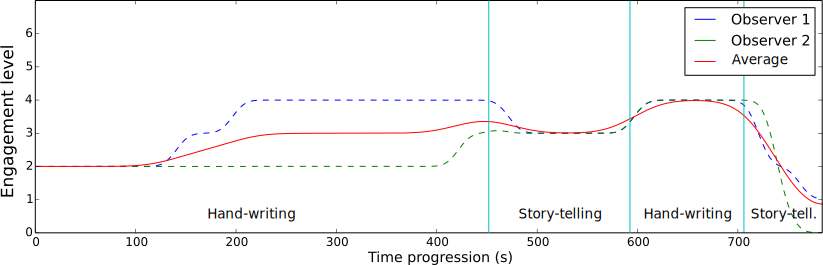
\includegraphics[width=0.9\linewidth]{engagement}
%    \caption{\small Engagement level of one child, manually annotated by two judges
%        over a 13 min long interaction (Cronbach’s alpha test: $\alpha = .82$,
%        good inter-judge agreement). 0 means ``complete disengagement from the
%        task'', 6 means ``full engagement''. The vertical lines represent activity
%    switches between handwriting teaching and story-telling (used as a
%    disturber).}
%    \label{engagement_level}
%\end{figure}

\begin{table}[h!]
    \centering
    \caption{\textbf{Levels of with-me-ness}. Percentage of interaction time
        during which the child was effectively focusing his/her attention on the
        task. The six children are those from the second study at School A.
        Interaction duration: M = 19.6 min, SD = 1.58. Results
        taken from~\cite{lemaignan2016realtime}.}

    \begin{tabular}{p{1cm}cccccccc}
        \toprule
        Child & 1 & 2 & 3 & 4 & 5 & 6 & {\bf M} & {\it SD} \\
        \midrule
        $\mathcal{W}$ & 79.4\% & 81.6\%  & 90.5\% & 87.9\% & 90.7\% & 80.9\% & {\bf 85.2\%} & {\it 5.1} \\ 
        \bottomrule
    \end{tabular}
    \label{tab:results-with-me-ness}
\end{table}

We also conducted a quantitative assessment of the engagement levels of the
children. Table~\ref{tab:results-with-me-ness} reports the levels of
\emph{with-me-ness} of the children during the second study at school A.
\emph{With-me-ness} is a quantifiable precursor of engagement: it measures the
percentage of time spent by the child focusing onto the task at end. It was
first devised in the context of computer-supported
learning~\cite{sharma2014me}, and we have previously studied its applicability to
human-robot interaction and formalized the exact methodology
in~\cite{lemaignan2016realtime}\footnote{Note that with-me-ness is a metric that
allows real-time computation by the robot itself: while we did not yet make
use of it, it would allow the robot to detect possible disengagements, and
eventually address them by adapting its physical behaviour, switching to
different activities, etc.}.

The average with-me-ness is well above 80\%, and confirms that the children
where very much engaged into these 20 minutes of interaction with the robot,
paying close attention to the task.

The other three experiments (the group study at the surgery and the two
case-studies) provide further qualitative assessment of engagement over longer
interaction periods. In particular, as reported hereafter, the two 4-weeks long
case studies that have been conducted so far show that our system can sustain
children' engagement over durations (5 hours) that are closer to what is
expected to have an impact in a real therapeutic context.

%%%%%%%%%%%%%%%%%%%%%%%%%%%%%%%%%%%%%%%%%%%%%%%%%%%%%%%%%%%%%%%%%%%%%%%%%%%%%%%%%%%
\subsection{Study: How Children Take on the Role of a Teacher}\label{normandie}

\paragraph{Context, Study Design}

\begin{inparaenum}
This experiment was conducted to study \item how easily children with actual
deficit take on the role of a teacher, and \item if they engage \emph{seriously}
in this role.
\end{inparaenum}

The experiment took place at the surgery of an occupational therapist in
Normandy, France. Eight children participated, all showing troubles with
handwriting acquisition: Valérie (7 years old), Antoine (6.5) and Johan
(7) are under the care of the occupational therapist. Émilien (8) and Mathieu (7)
are repeating their school year because of writing difficulties. Mona (6) and
Adèle (8) are both ranked at the bottom of their respective classes in writing
activities. Nicolas (7) is under the care of a neurologist, and has been
diagnosed with specific language impairment. Given their school level, all those
children would be expected to know how to correctly shape cursive letters. 

Over a period of two weeks, each child attended three time a one hour long
session, except for Adele and Mona who only attended one session. The
experimenter role was limited to the explaination of the rules of the game and
the basic tablet usage. For this experiment, the children were provided with two
tablets: one to choose the word (or single letter) to teach to the robot, one
used to write. We also provided templates of the cursive letters, where the
children to ask for.

We only provided the children with minimal explanations on the task (they would
have to help the robot to improve its writing style), so as to assess if and how
children would naturally take on the role of the teacher, and how seriously they
engaged into helping the robot.

This assessment was carried through two additional buttons on the tablet: a
green ``thumbs up'' and a red ``thumbs down''. The children were told to use
them to evaluate the robot's improvements (``thumb up'' being a way to give
positive feedback while ``thumb down'' would be convey negative feedback). Our
assessment builds on the hypothesis that the more the child provides feedback to
the robot with the green/red buttons, the more he/she assumes the role of a
teacher. Then, by correlating the feedback with the actual performance of the
robot, we can measure to what extend the child was seriously assuming his/her
role: since the child knows what a correct letter should look like, if his/her
feedback does not correlate with the actual performance, the child was likely
engaged into a playful instead of serious role-playing.


\paragraph{Results}

All children maintained their engagement during the whole sessions. They
provided on average 42 demonstrations per session. All children used the
feedback buttons and had preference to give positive feedback the robot (99
``thumb up'' \vs 33 ``thumb down'' were recorded). 

As the children participated at most 3 hours of interactions spanning over two
week, we did not attempted to measure possible handwriting improvements by the
children, and instead we focused on the possible correlation between the
children's feedback and the robot's progression.  We estimated the robot's
progression as the difference between a starting score (score of the first
robot's try when children have chosen a new word/letter to work on) and the
current robot's score (after being taught by the child). The score is calculated
as the average of euclidean distance between robot's try and a reference
allograph over all letters of the word. Those references for letter allographs
where drawn by us beforehand, taking inspiration in education.com cursive
letters
template\footnote{\url{http://www.education.com/slideshow/cursive-handwriting-z/}}.
Let $P_i$ be the estimated progression of the robot at time $ i$. Of course, if
the child chose to switch to a new word at time $ j$ , we have $ P_{j}=0$ and
clearly $ P_0=0$.  To measure whether the fact that the child was rewarding the
robot when it was progressing was significant or not, we generated 10000 times
the same number of reward/punishment but accorded at random times. Let $ R_i^n$
be the $n^{th}$ generated evaluation at time $ i$ ($ R_i^n = 0$ if no evaluation
occurred at time $ i$ , $ R_i^n=1$ if a reward occurred at time $i$ and
$R_i^n=-1$ if a punishment occurred at time $i$), and $\overline{R}_i$ be the
actual evaluation at time $i$. For each $n^{th}$ generated sequence of
evaluation, we compute a score of evaluation: $$ S^n = \sum\limits_i{R_i^n
P_i}$$ Then we can estimate the p-value $p$ of the actual score: $$ \overline{S}
= \sum\limits_i{\overline{R}_i P_i}$$ given the distribution of the generated
scores $\left(S^n\right)_n$, which is assumed to be Gaussian: 

$$
p(\overline{S})= \mathbb{P}{\left[X>\overline{S}\right]} = 1-\phi{\left(\frac{\overline{S}-\mu}{\sigma}\right)}
$$

where $\phi$ denotes the cumulative distribution function of the standard normal
distribution, $\mu$ the mean and $\sigma$ the deviation of the generated scores
$\left(S^n\right)_n$.  As a result, we found that 5 of the 8 children obtained a
score of evaluation significantly hight ($p(\overline{S})<0.05$). Score of
evaluation p-values of each child is reported in the second-to-last column of
Table~\ref{table:scores}.

We also studied correlation between children's evaluations and their own
progression. The analysis was conducted in the same way, using distances between
children demonstrations and reference allographs to compute children
progressions.  3 of 5 children that played ``seriously" obtained score of
evaluation of their own progression significantly high (last column of
Table~\ref{table:scores}). For those children, it seems that the robot was
reflecting their own performances, and while they were judging the robot
positively (three times more rewards than punishments) they were actually
evaluating themselves.

\begin{table}
    \centering
    \begin{tabular}{|c|c|c|c|c|c|}
        \hline
        child & demo & rew & pun & p(robot) & p(child)\\ \hline
        Valérie & 127 & 24 & 6 & 2.4e-03 & 5.5e-02\\ \hline
        Émilien & 223 & 20 & 9 & 1.7e-01 & 3.5e-01\\ \hline
        Mathieu & 131 & 10 & 3 & 3.8e-03 & 7.9e-03\\ \hline
        Johan & 98 & 10 & 5 &  1.5e-01 & 3.8e-01\\ \hline
        Nicolas & 115 & 16 & 4 & 5.3e-04 & 2.7e-03\\ \hline
        Antoine & 83 & 10 & 3 & 3.1e-02 & 6.0e-01\\ \hline
        Adèle & 35 & 4 & 2 & 5.0e-02 & 3.7e-02\\ \hline
        Marie & 40 & 5 & 1 &  5.4e-01 & 2.0e-01\\ \hline
    \end{tabular}
    \caption{\small results of evaluations. demo: number of demonstrations provided by
        the child over all session. rew: number of rewards accorded by
        the child. pun: number of punishments. p(robot): are the evaluations
        significantly corresponding to the progression of the robot ? p(child): are the
        evaluations significantly corresponding to the child's own
progression ?}
    \label{table:scores}
\end{table}

%%%%%%%%%%%%%%%%%%%%%%%%%%%%%%%%%%%%%%%%%%%%%%%%%%%%%%%%%%%%%%%%%%%%%%%%%%%%%%%%%%%
\subsection{Case Study 1: Vincent}

\paragraph{Context, Study Design}

For the first case study, we invited and followed Vincent, a six years old
child, once per week over a period of a month. Our primary aim was to address the
question of whether we can sustain Vincent's engagement and commitment to the
writing activity over such a period.

\begin{figure}
    \centering
    \includegraphics[width=0.5\linewidth]{diego}
    \caption{\small Vincent correcting {\sc nao}'s attempt by rewriting the
        whole word. Empty boxes are drawn on the screen to serve as template for the child
        and to make word segmentation more robust.}
    \label{fig:diego}
\end{figure}

The study took place at our laboratory (Figure~\ref{fig:diego}), and we chose to
design the activity around a storyline meant to be attractive for a 6 years old
boy: one of our {\sc nao} was away for a mysterious scientific mission, and it
needed the support of another one -- which would remain at the lab -- to interpret
curious pictures that were sent every week. Vincent had to help the second robot
understanding the pictures, and since the two robots had somehow beforehand
agreed to communicate with ``letters written like humans'' (\ie handwritten),
Vincent also had to help the robot to write good looking letters (because, well,
this robot was terrible at writing!) The experimental setup was similar to
Figure~\ref{experimental_setup}, except that Vincent had to tell the robot what
to write with small plastic letters (visible behind the robot on Figure~\ref{fig:diego}).

To complement the intrinsic motivation of helping a robot to communicate with another one, we
gradually increased the complexity of Vincent's task to keep it challenging and
interesting (the first week: demonstration of single letters; the second week:
short words; the third week: a full letter -- Figure~\ref{fig:stimuli}).

The last session was set as a test: the ``explorer'' robot
had come back from its mission and it actually challenged the other robot in
front of Vincent: \emph{``I don't believe you wrote yourself these nice letters that I
received! Prove it to me by writing something in front of me!''} This situation
was meant to evidence the Protégé effect: by judging the other robot's
handwriting, the ``explorer'' robot would implicitly judge Vincent's skills as
teacher, and in turn, Vincent's handwriting.

\paragraph{Results}

\begin{figure}
    \centering
    \subfigure[Initial text, generated by the robot]{
        \includegraphics[height=6cm]{diego-initial-letter}
    }
    \subfigure[Final text, after training with Vincent]{
        \includegraphics[height=6cm]{diego-final-letter}
    }

    \caption{\small (French) text generated by the robot, before and after a one
        hour long interaction session with the child. The red box
        highlights one instance of striking improvement of the robot's
        handwriting legibility.}

    \label{fig:stimuli}
\end{figure}

Over the whole duration of the study, Vincent had provided 154 demonstrations to the robot, and he remained
actively engaged over the four weeks. The story was well accepted by the child and
he seriously engaged into the game. After the first week, he showed good
confidence to play with the robot and by the end of the study he had built
affective bonds with the robot, as evidenced by several letters he did send to the
robot \emph{after} the end of the study (one of them four months later) to get
news. This represents an initial validation of our hypothesis: our system can effectively keep a
child engaged with the robot for a relatively long periods of time (about 5
hours spread over a month).

No hard conclusion can be drawn in terms of actual handwriting remediation: we did
not design this study to formally assess possible improvements. However, as
visible on Figure~\ref{fig:stimuli}, Vincent was able to significantly improve
the robot's skill, and post-hoc interviews revealed that he acknowledged that he
was the one helping the robot. In that respect, Vincent realized that he was
``good enough'' at writing to help someone else. Quoting the mother a week
after the end of the experiment: ``Vincent's handwriting has changed over the
last weeks, going from a mix of standalone and cursive letters to full words in
cursive. This requires a lot of efforts and concentration from him, but he did
succeed during the sessions with the robot as he knew he had to show a
consistent writing to the robot''.


%%%%%%%%%%%%%%%%%%%%%%%%%%%%%%%%%%%%%%%%%%%%%%%%%%%%%%%%%%%%%%%%%%%%%%%%%%%%%%%%%%%
\subsection{Case Study 2: Thomas}

\paragraph{Context, Study Design}

The second long-term study was designed with the help of an occupational therapist in
Geneva and aimed at deploying the system for the first time on a real
therapeutic case.

Thomas is a 5.5 years old child, under the care of this occupational therapist. He
has been diagnosed with visuo-constructive deficits, which translate into
difficulties for him to consistently draw letters. Besides, focusing on a task
is difficult for Thomas, who tends to rapidly shift his attention to other
things. Since the robot's learning algorithm requires repeated demonstrations of
similarly shaped letters to converge, the occupational therapist was especially
interested in observing if the robot would induce a strong enough motivation for
Thomas to focus on producing regular, consistent letters, thus overcoming his
deficit.

The experiment took place at the therapist's surgery (four sessions spanning
over 5 weeks). Contrary to Vincent's experiment, we chose not to introduce any
storyline beyond a simple prompt (``the robot wants to participate to a robotic
handwriting contest, will you help him to prepare?''), only provided during the
first session. Hence, we also tested during this case-study if the robot (and
the Protégé effect) would induce by itself a strong enough intrinsic motivation to
keep the child engaged over the five weeks.

\begin{figure}
    \centering
    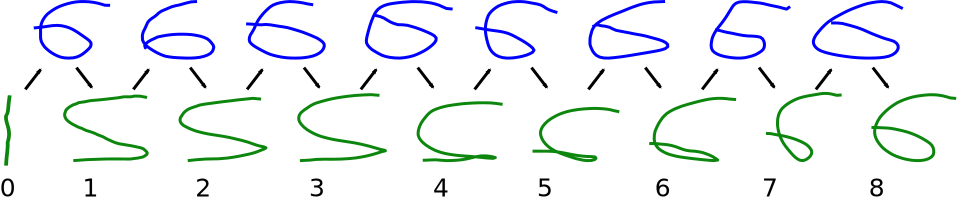
\includegraphics[width=0.9\linewidth]{learning_6_demos}

    \vspace{1em}

    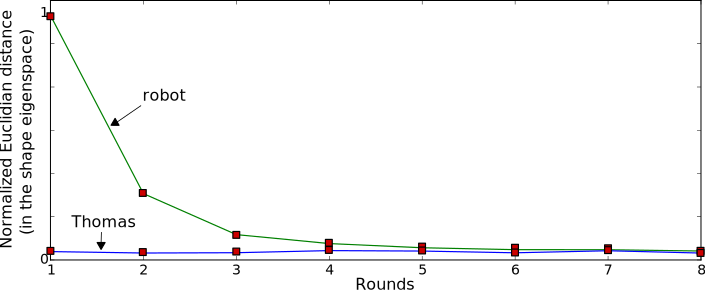
\includegraphics[width=0.7\linewidth]{learning_6_distances}
    \caption{\small Demonstrations provided by Thomas for the number ``6'' (top row) and
        corresponding shapes generated by the robot. The plot beneath shows the distance
        (in the eigenspace of the shape) between Thomas demonstrations, the
        robot's attempts and our reference shape. After eight demonstrations,
        Thomas decided that the robot's ``6'' was good enough, and switched to
    another character. In that respect, he was the one leading the learning
process of the robot.}
    \label{learning_6_demos}
\end{figure}


The occupational therapist had recently carried activities with Thomas about
writing numbers, so we decided with her to focus on these as well: Thomas would
use a secondary tablet to tell the robot what number to write, and would then
correct the robot's attempts like in the other experiments.
Figure~\ref{learning_6_demos} shows the attempts/corrections cycles that
occurred during one of the session, on the number ``6''.

%Before the experiment, Thomas was working on writing numbers with the therapist.
%Hence we decided to turn the CoWriter activity to teach numbers to the robot.
%Build on existing iPad applications actually used by occupational therapists
%(Dawson Toth's \emph{ABC's Writer}), we designed an Android application for
%pre-test and post-test. It consisted in drawing numbers following an helping
%pattern, that becomes more fine with levels in order to increase
%difficulty~\ref{fig:abc-writer}.

Since Thomas would frequently draw mirrored numbers, or hard-to-recognize
shapes, the learning algorithm of the robot initially tended to converge towards
meaningless scribblings. We addressed this issue by having the robot to
\emph{refuse} allographs that were too far from the reference shape (the robt
would instead say \emph{``I'm
not sure to understand what you are drawing...''}), so that the child had to
pay good attention to what he would demonstrate to the robot. Also, to make
the robot's progresses evident, we modified the initialization step of the
learning algorithm to start with a roughly vertical stroke instead of a
deformed number (see the initial state on Figure~\ref{learning_6_demos}).

%\begin{figure}
%    \centering
%    \includegraphics[width=0.9\linewidth]{abc-writer}
%    \caption{\small Screenshot of the Android application developed to be used as
%    pre-test and post-test: the child must follow with his finger the path of
%the letter or number. We count the number of times the finger goes outside of
%the red-bordered area.}
%    \label{fig:abc-writer}
%\end{figure}
%

\paragraph{Results}

Despite his attention deficit, Thomas was able to remain engaged in the activity during more than
forty minutes in each session. In total, 55 allographs out of 82 
demonstrated by the child were acceptable considering our threshold (with a
progressive improvement from 13 out of 28 in the first session up to 26 out
of 29 in the last session).

As soon as Thomas understood that the robot was only accepting well-formed
allographs, he started to focus on it and he would typically draw 5 or 6 times
the number before actually sending to the robot (the tablet lets children
clear their drawing and try again before sending it). According to
the therapist, it was the first time that Thomas would correct himself in such a
way, explicitly having to reflect on how \emph{another agent} (the robot) would
interpret and understand his writing. Figure~\ref{Thomas_progress} shows how
he gradually improved his demonstrations for two different numbers, according to the
metric we used to make the robot accept/refuse samples.

Since the robot's handwriting started from a simple primitive (a stroke), each
time Thomas succeeded to have his demonstration accepted by it, the robot's
improvement was clearly visible (as shown in Figure~\ref{learning_6_demos}).
This led to a self-rewarding situation that effectively supported Thomas'
engagement.

\begin{figure}
    \centering
    \subfigure[Number ``2'']{
        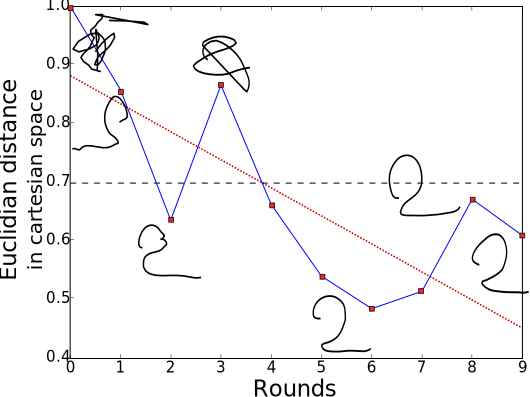
\includegraphics[width=0.45\linewidth]{henry2}
    }
	\subfigure[Number ``5'']{
        \includegraphics[width=0.45\linewidth]{henry5}
    }
    \caption{\small Normalized distance between Thomas' demonstrations and
        reference allographs for the numbers ``2'' and ``5''. The horizontal
        dashed line correspond to the threshold for the robot to accept a
        demonstration. Thomas' progress is visible on these figures: we find a
        significant negative regression equation ($r=-0.023, F(1,19)=8.69,
        p<.02$, adjusted $R^2=.461$) for the number ``2'' (dotted red line),
        indicating that Thomas' shapes are getting closer to the reference. The
        regression is not significant for the number ``5'', but we can observe
        that after about 10 repetitions, all the demonstrations are deemed of
        acceptable quality by the robot.  }

    \label{Thomas_progress}
\end{figure}



%%%%%%%%%%%%%%%%%%%%%%%%%%%%%%%%%%%%%%%%%%%%%%%%%%%%%%%%%%%%%%%%%%%%%%%%%%%%%%%%%%%
%%%%%%%%%%%%%%%%%%%%%%%%%%%%%%%%%%%%%%%%%%%%%%%%%%%%%%%%%%%%%%%%%%%%%%%%%%%%%%%%%%%
\section{Conclusion}

We believe that this research provides a novel perspective on educative
robots at several levels. We show that:

\begin{itemize}
    \item robots in an educative context are \textbf{relevant and effective
        beyond STEM} (Science, Technology, Engineering and Mathematics)
    \textbf{teaching},

    \item we can successfully \textbf{transpose the well-established
        \emph{learning by teaching} paradigm} from education sciences to
        robotics, even in a \textbf{complex form}: handwriting is difficult
        physical skill, the robot learns and interact autonomously, the child is
        responsible not only for the teaching but also for the teaching
        orchestration by managing the turn taking and the progression of the
        activity,

    \item blending machine-learning techniques with human-robot interaction
        allows for building a \textbf{believable agent}, that induces
        \textbf{social commitment},

    \item this proves essential to \textbf{sustain a long-term interaction} (several
        hours) around a fundamentally routine -- yet challenging -- educational
        task (handwriting learning),

    \item besides, the social commitment induces a \textbf{cognitive engagement}
        of the child with the robot which is \textbf{a key learning lever} as
        its elicits \textbf{reflective, meta-cognitive mechanisms on the
        learning task}.
\end{itemize}

As we show through extensive experimental validation, these claims are not just
words: we have effectively deployed robots on the field, with children suffering
actual handwriting impairments. Our results are promising in terms of sustaining
the interest and attention of children on otherwise boring writing exercises,
and we evidence clear handwriting improvements.

It is however still early to quantify the lasting effects of this remediation:
handwriting is a complex cognitive skill, that builds on many individual and
social factors. Self-confidence is one of them. We expect that our
approach that endows the child with the role of a teacher who can help a robot,
may help some children to recover self-esteem and self-confidence. However the
experiments that we have conducted so do not allow us to confirm this
hypothesis, and more research need to be conducted in this direction.


\paragraph{Possible Ethical Concerns} Two aspects of this research ought to be
discussed in term of their possible ethical implications: the perceived role of
the robot \textit{vis-à-vis} the teacher, and the implications of the
mentor-protégé relationship for children, especially vulnerable ones.

The place and role of the robot \textit{vis-à-vis} the teacher can be
questioned: as we see it, the role of the robot within the classroom (or at the
therapist's surgery) does not infringe upon the role of the adult (teacher or
therapist).  The core of the \emph{learning by teaching} paradigm relies on the
child becoming the teacher of an underperforming pupil (the robot): from that
perspective, the robot does not replace the teacher, on the contrary. It plays a
different role in the classroom, which happen to be novel as well: the robot is
the \emph{least} performing student, and still a very patient, always eager to
improve, one.

The importance of the adult is further supported by our experiments: even with
an autonomous, nominally performing robot, to put the teacher's clothes on
remains (expectedly) difficult for 5-6 years old children, and during the
experiments we conducted, the adult always played a key role at prompting the
child to give feedback to the robot or to move to the next letter or word.  At a
higher orchestration level (and as reported in the two case studies with Vincent
and Thomas), the educational scenarios were also always designed and monitored
by the adults.

We initially envisioned our system to be run in the back of a classroom with one
child: this would have allowed an individual, face-to-face remediation approach,
not otherwise tractable for a teacher with 20 pupils.  This is however unlikely
to happen soon. In our experience, the teacher keeps such an important role that
the interaction (and the learning!) would hardly occur if the child is left
alone (or even semi-alone). We can therefore reassure teachers: robots are not
going to replace them any time soon.

The implication of the mentor-protégé relationship on the children is less
clearly understood. The children can establish strong affective bonds with the robot (as
witnessed by the letter sent by Vincent several months after he interacted with
the robot), but we are not yet able to precisely characterize these bonds. The
ethical implication of the mentor-protégé relationship have been explored before
in the context of human teaching~\cite{brad1999mentor,wendelyn2008context}, but
they mostly look at the question from the perspective of the protégé, whereas in our
case, the child is the mentor. As such, relatively little is known on the
psychological implications for a child to commit in helping a robot, and as
advocated by Belpaeme and Morse~\cite{belpaeme2010time}, we likely need to first
gain more field experience before being able to draw conclusions.

Beyond handwriting, we however do believe that this work provides a novel
perspective on the role for robots in the field of education. \emph{Learning by
teaching} is a powerful paradigm because of not only its pedagogical efficacy,
but its potential to positively impact the child's motivation and self-esteem.
We hope that this article shows that this is a very relevant context of use for
robots: when facing a child with school difficulties, robots can play the role
of a naïve learner which neither adults nor peers -- because of the social
effects it would induce -- can convincingly play.


%%%%%%%%%%%%%%%%%%%%%%%%%%%%%%%%%%%%%%%%%%%%%%%%%%%%%%%%%%%%%%%%%%%%%%%%%%%%%%%%%%%
%%%%%%%%%%%%%%%%%%%%%%%%%%%%%%%%%%%%%%%%%%%%%%%%%%%%%%%%%%%%%%%%%%%%%%%%%%%%%%%%%%%
\section*{Acknowledgments}

We warmly thank all the children, teachers and staff of the International School
of Geneva, the Institut Florimont and the Haut-Lac school for their
participation and support. We express our great gratitude to Anne Gossin and [TBD] for
inviting us to their surgery, for their involvement in the experiments and for
bearing with our disruptive robots. And finally, we want to say a very special \emph{Thank
you!} to Vincent, Thomas, Valérie, Émilien, Mathieu, Johan, Nicolas, Antoine,
Adèle and Marie: by spending several hours being patient teachers for our
robots, you have paved the way for what may become tomorrow a new way of
learning how to deal with all these letters and words!

This research was partially supported by the Funda\c{c}\~{a}o para a Ci\^{e}ncia
e a Tecnologia (FCT) with reference UID/CEC/50021/2013, and by the Swiss
National Science Foundation through the National Centre of Competence in
Research Robotics.

\bibliographystyle{abbrv}
\bibliography{biblio}


\end{document}
